\documentclass[12pt, oneside]{article}
\usepackage[letterpaper, margin=1in, headsep=0.5in]{geometry}
\usepackage[english]{babel}
\usepackage[utf8]{inputenc}
\usepackage{amsmath}
\usepackage{amsfonts}
\usepackage{amssymb}
\usepackage{tikz}
%\usepackage{venndiagram}

\usepackage{fancyhdr}
\pagestyle{fancy}
\fancyhf{}
\rhead{\thepage \\Name: \hspace{1.5in}.\\}
\lhead{BECA / Dr. Huson / 11.1 IB Math SL\\* 23 May 2018 \\*\textbf{Homework: Statistics, exponential, \& polynomial functions
}}

\renewcommand{\headrulewidth}{0pt}

\begin{document}


\begin{enumerate}


\item In an arithmetic sequence, the first term is 5.3 and the second term is 3.7.
\begin{enumerate}
    \item Find the common difference.
        \begin{flushright}[2]\end{flushright}
    \item Find the tenth term. (use the formula)\\[50pt]
        \begin{flushright}[2]\end{flushright}
    \item Find the sum of the first fifteen terms of the sequence. (use the formula)\\[50pt]
        \begin{flushright}[2]\end{flushright}
\end{enumerate}

\item Simplify the expression $\sqrt{x^6 y^2}$.\\*[60pt]
        \begin{flushright}[2]\end{flushright}

\item Carlos puts \$12,500 into an investment account with interest compounded continuously. If the annual interest rate is 3.15\% what is the balance after 7 years, to the nearest dollar. %\\[80pt]
        \begin{flushright}[5]\end{flushright}

\newpage
\item Given the function $f(x)=-x^3+2x^2+5x-6$.
  \begin{enumerate}
      \item Write down the $y$-intercept.
          \begin{flushright}[1]\end{flushright}%\\*[10pt]
      \item Find the $x$-intercepts.%\\*[20pt]
          \begin{flushright}[2]\end{flushright}

      \item Graph the function on the grid below, carefully passing through the correct intercepts.
          \begin{flushright}[3]\end{flushright}
      \item What is the maximum value of $f(x)$ over the domain $0 \leq x \leq 5$, to three significant figures?
          \begin{flushright}[2]\end{flushright}
  \end{enumerate}
    \begin{center}
      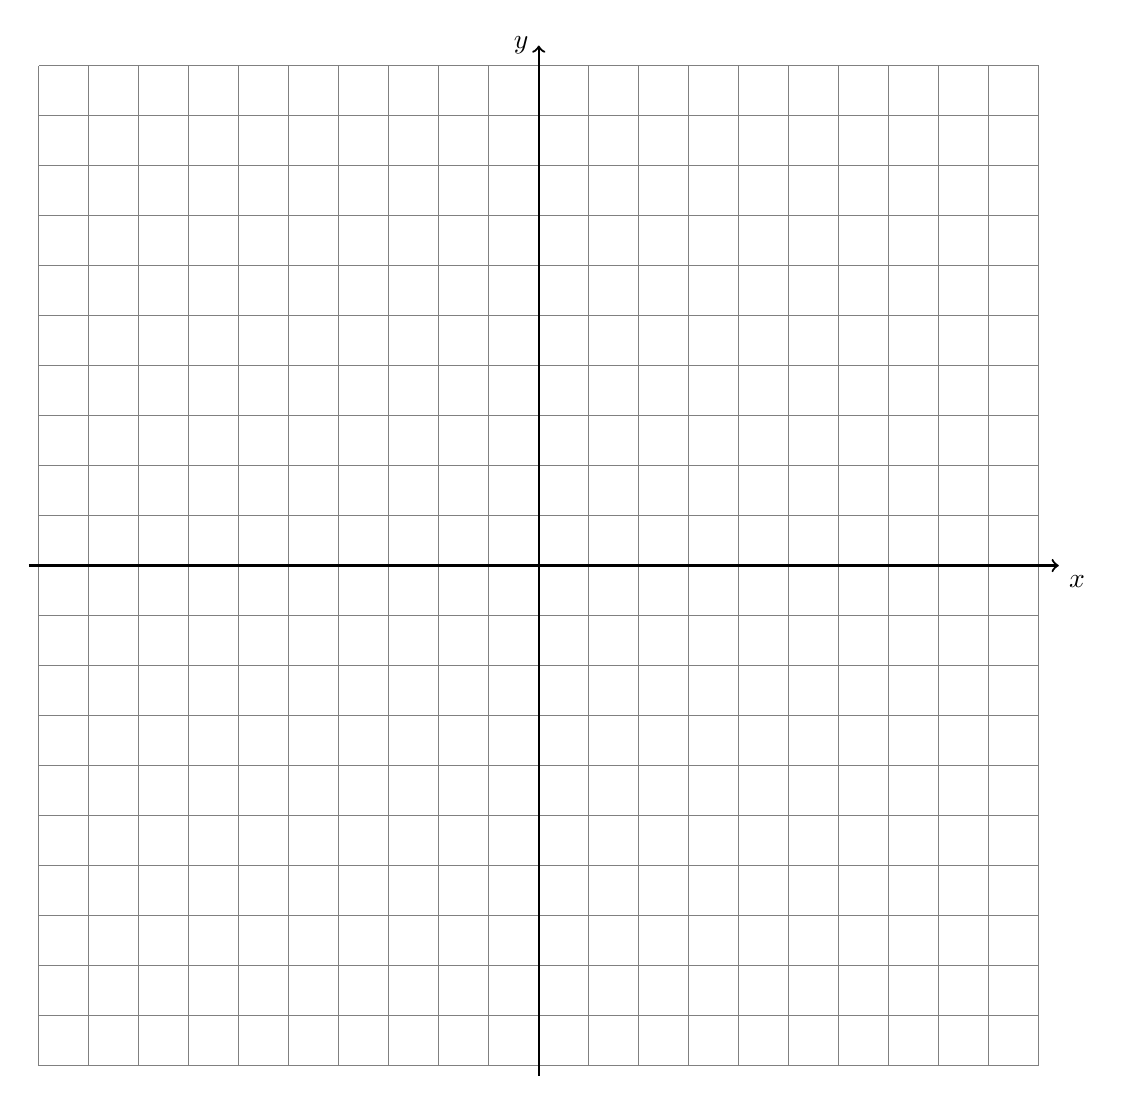
\begin{tikzpicture}[scale=.635]
        \draw [help lines] (-10,-10) grid (10,10);
        \draw [thick, ->] (-10.2,0) -- (10.4,0) node [below right] {$x$};
        \draw [thick, ->] (0,-10.2)--(0,10.4) node [left] {$y$};
      \end{tikzpicture}
    \end{center}

\newpage

\item The expression $(x + a)(x - b)$ can not be written as
\begin{enumerate}
    \item $x(x + a)- b(x + a)$
    \item $x^2 + ax - bx - ab$
    \item  $x^2 + (a - b)x + ab$
    \item $x(x - b)+ a(x - b)$
\end{enumerate}
        \begin{flushright}[2]\end{flushright}

\item Consider a geometric sequence where the first term is 112 and the second term is 84.
\begin{enumerate}
    \item Find the common ratio, $r$.\\[20pt]
        \begin{flushright}[1]\end{flushright}
    \item Find the seventh term.\\[80pt]
        \begin{flushright}[2]\end{flushright}
    \item Find the least value of $n$ such that the $n$th term of the sequence is less than 20. \\[80pt]
        \begin{flushright}[3]\end{flushright}
\end{enumerate}

\newpage
\item Algebraically determine the values of $h$ and $k$ to correctly complete the identity stated below.
\[2x^3-5x^2+5=(x-2)(2x^2+hx+2)+k\] \\[2in]
        \begin{flushright}[4]\end{flushright}

\item Three consecutive terms of a geometric sequence are $x-4$, 6, and $x+5$.\\
Find the possible values of $x$.\\[3in]
    \begin{flushright}[6]\end{flushright}

\newpage
\item A bank account earns interest at a continuous interest rate of 1.04\% per year. The initial deposit is \$175. Which function models the value of the balance? \qquad [2]
\begin{enumerate}
    \item $P(t)=175 \cdot 1.01045^{t}$
    \item $P(t)=175 (1+0.03925)^{t}$
    \item $P(t)=175 \cdot 1.03925^{t}$
    \item $P(t)=175 \cdot e^{0.04t}$
\end{enumerate}
    %\begin{flushright}[5]\end{flushright}


\item Write $\sqrt[3]{a^5} \div a^{\frac{2}{3}}$ as an expression with positive, integer exponents.\\*[40pt]
    \begin{flushright}[3]\end{flushright}

\item The function $p(t)=110e^{0.045t}$ models the population of a city, in millions, $t$ years after 2010.
\begin{enumerate}
    \item Initially, as of 2010, what is the population in millions?%\\[20pt]
        \begin{flushright}[1]\end{flushright}
    \item What is the annual continuous rate, expressed as in percent, that the population increases?%\\[10pt]
        \begin{flushright}[1]\end{flushright}
    \item Find the population in 2015, rounded to the nearest million.\\[60pt]
        \begin{flushright}[2]\end{flushright}
    \item In what year will the population be approximately 165 million?
        \begin{flushright}[2]\end{flushright}
\end{enumerate}



\end{enumerate}
\end{document}
